%\documentclass[12pt]{article}
%\usepackage[a4paper, margin=1in]{geometry} 
%\usepackage{graphicx} 
%\usepackage{hyperref}
%\usepackage{float}
%\usepackage{multicol}
%\usepackage{multirow}
%\usepackage{amsmath}
%\usepackage[font=small, labelfont=bf]{caption}
%
%\begin{document}

%
% Hidden Markov model
%
\subsection{Hidden Markov model}
An HMM (hidden Markov model) is a probabilistic graphical model that assumes a Markov property. It contains two different types of probabilities: transition and emission probabilities.

\begin{figure}[H]
  \centering
      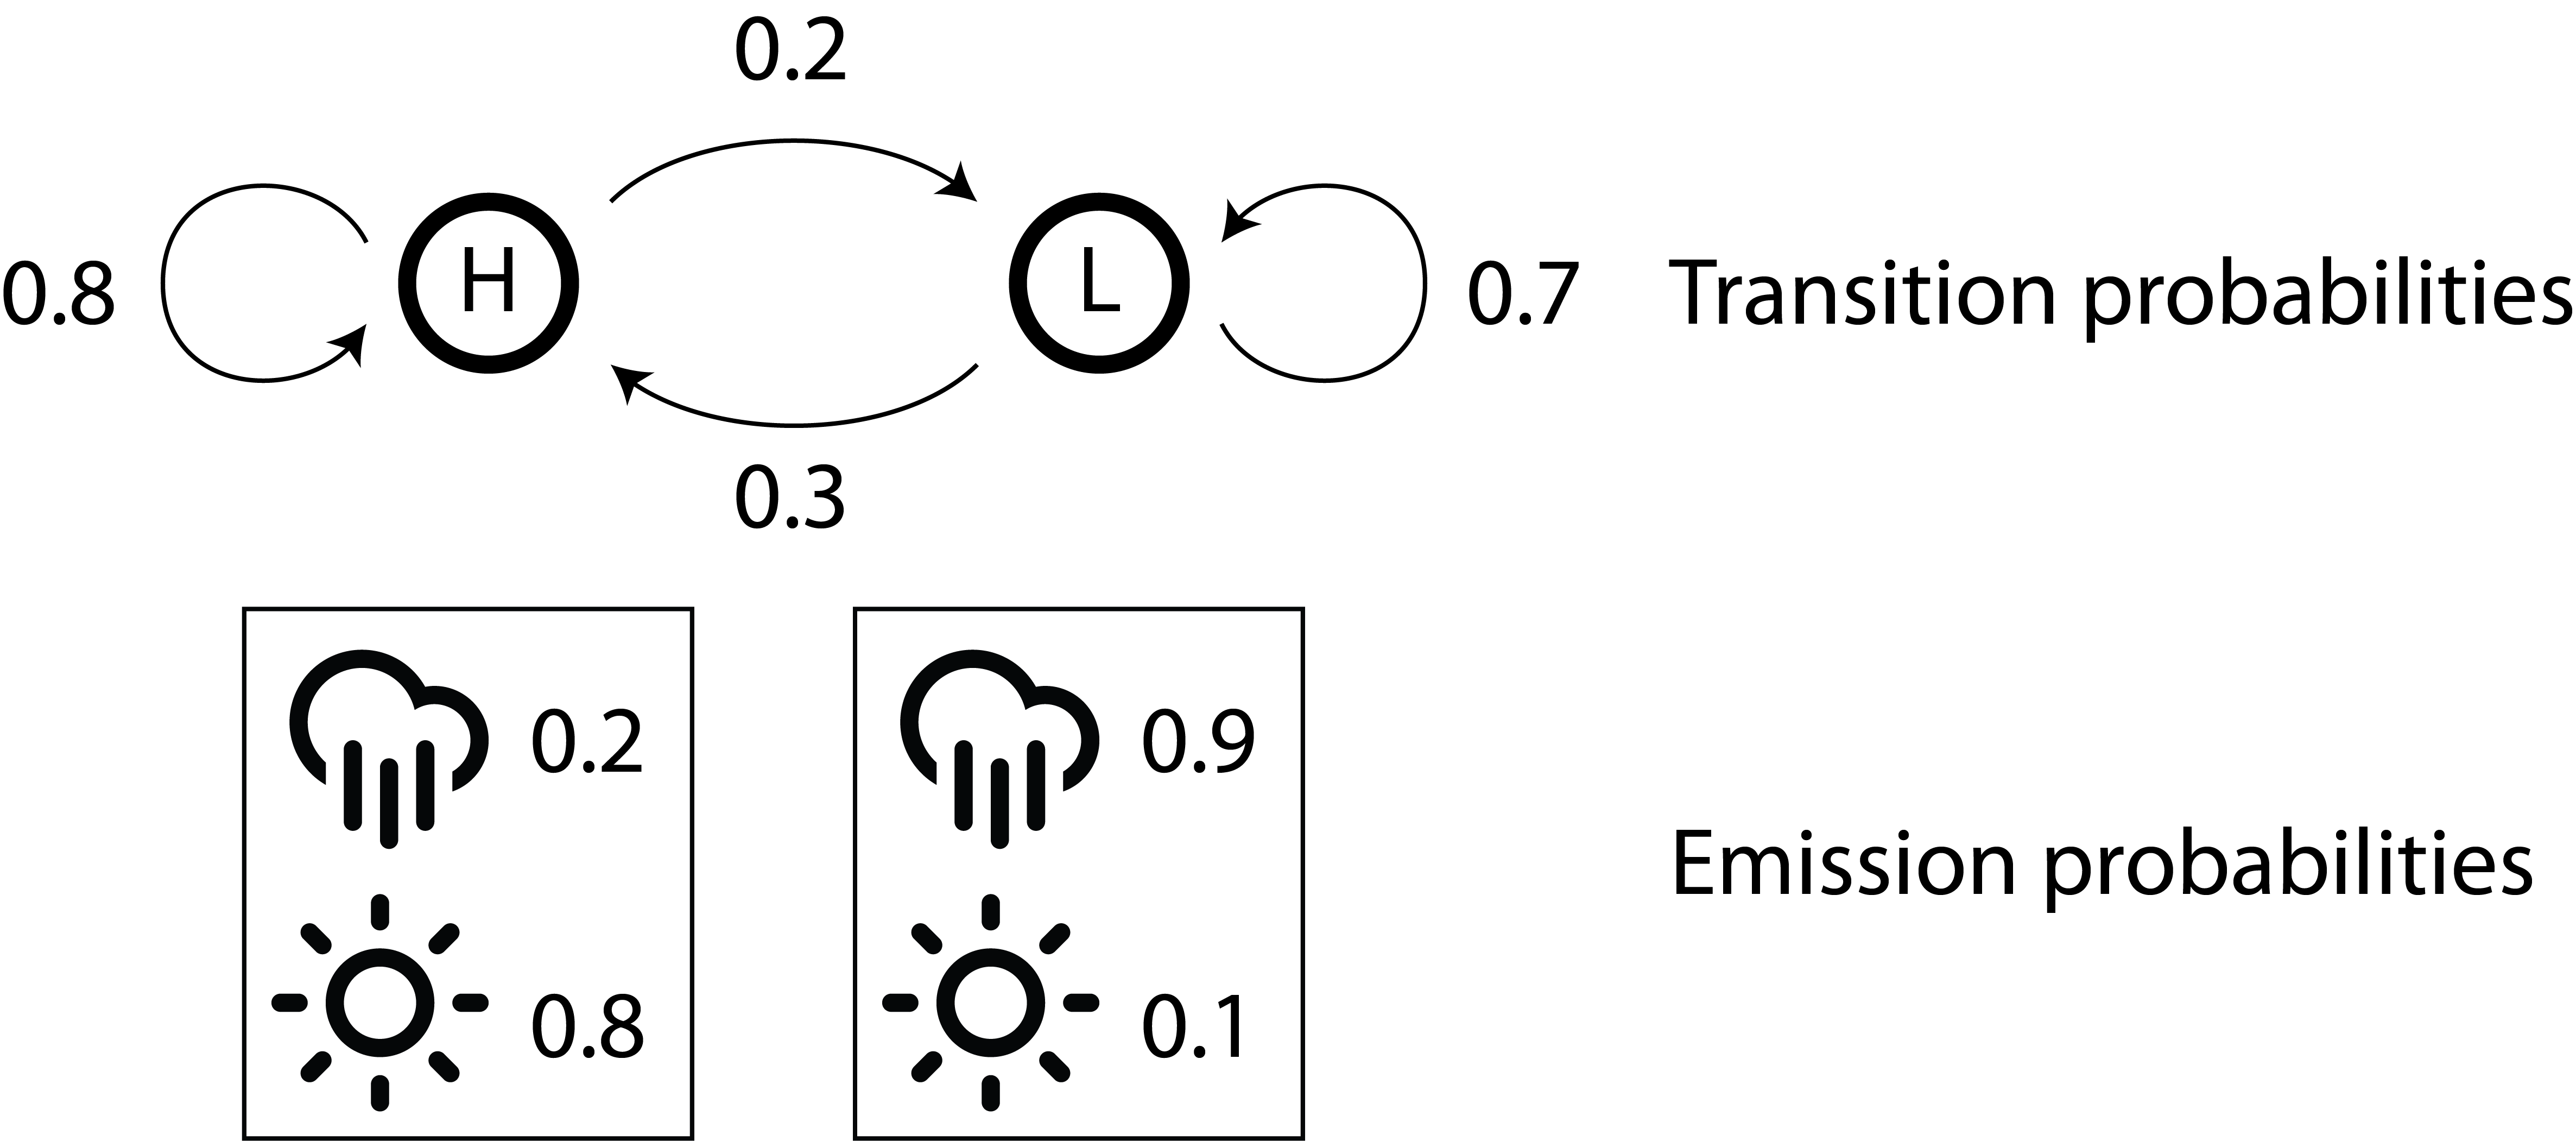
\includegraphics[width=0.5 \textwidth]{fig13/HMM_example.png}
  \caption{HMM for weather conditions}
\end{figure}

%
% Example of HMM probability calculation
%
\subsubsection*{Example of HMM probability calculation}
Calculate the probability when the observed weather conditions are (Sunny, Sunny, Sunny) and the corresponding states are (L, H, H). Assume no particular prior distribution for the initial states. \\

$\begin{aligned}
&p(\mathrm{L}) \cdot  p(\mathrm{Sunny}|\mathrm{L}) 
\times p(\mathrm{H}|\mathrm{L}) \cdot  p(\mathrm{Sunny}|\mathrm{H}) 
\times p(\mathrm{H}|\mathrm{H}) \cdot  p(\mathrm{Sunny}|\mathrm{H}) \\
&= 0.5 \cdot 0.1 \times 0.3 \cdot 0.8 \times 0.8 \cdot 0.8 \\
&= 0.00768
\end{aligned} $

%
% Search and training of HMM
%
\subsubsection*{Search and training of HMM}
A dynamic programming is commonly used to search the most probable path, and an EM (Expectation-Maximization) algorithm is often used for training.

\begin{itemize}
\item Viterbi algorithm: A dynamic programming for searching HMM
\item Baum–Welch algorithm: An EM algorithm for training HMM
\end{itemize}

%
% Exercise \thesection.1
%
\subsubsection*{Exercise \thesection.1}
Use the transition and emission probabilities in the HMM above and calculate the probability when the observed weather conditions are (Rain, Rain, Sunny) and the corresponding states are (H, L, L). 

\bigskip 

\bigskip 

%\end{document}
